%!TEX root = ../../super_main.tex
\chapter{Gathering Sensor Data}
\label{cha:gathering_sensor_data}
\todo[inline]{Rikke: This chapter need some rework: ``Der er meget indforstået information i dette kapitel''}

A core feature of the platform, we are developing, is the ability to gather sensor data from the participants' devices. This chapter describes how this sensor data is structured, but also the functionality that ensures that we handle this gathering concurrently such that the collection of data from different sensors do not interfere.

%!TEX root = ../../super_main.tex

\section{The Campaign Model}
Conceptually, a \emph{snapshots} is a snippet of the reality (context) that a specific participants exists in, measured through the subjects devices along with a \emph{label}, describing this reality further. This label is used to define the reality in ways that available sensors cannot. By examining snapshots, and their labels, customers will be able to recognize patterns in measurements, and be able to see a correlation between sensor output and human dynamics. To see development of patterns in time, multiple measurements might be required. To facilitate this, a snapshot consists of a series of \emph{measurements}, each divided into \emph{samples}. To avoid collection redundant data, and wasting the participants resources, the customer must specify what sensors are required, the temporal properties of snapshots, and also how the data should be labeled. This is done through specifying a \emph{campaign}, which participants can contribute to. 
\\\\
One could imagine that a customer might be interested in finding a correlation between heart rate and movement patterns and the influence of alcohol. To do this, a customer would specify a campaign, which should collect information regarding sensors such as \emph{heart rate}, \emph{accelerometer}, and \emph{GPS location}. To know if the participants have consumed alcohol, the customer would specify that participants should indicate if they are, or have been, under the influence of alcohol at a specific time. When contributing information to this campaign, participants would submit snapshots matching this specification. An illustration of how these snapshots are structured can be seen in  \figref{fig:snapshot_example}. In this example, the participants are asked to label the snapshot by answering the question \emph{Are you under the influence by alcohol?}.

\begin{figure}[!htbp]
    \centering
    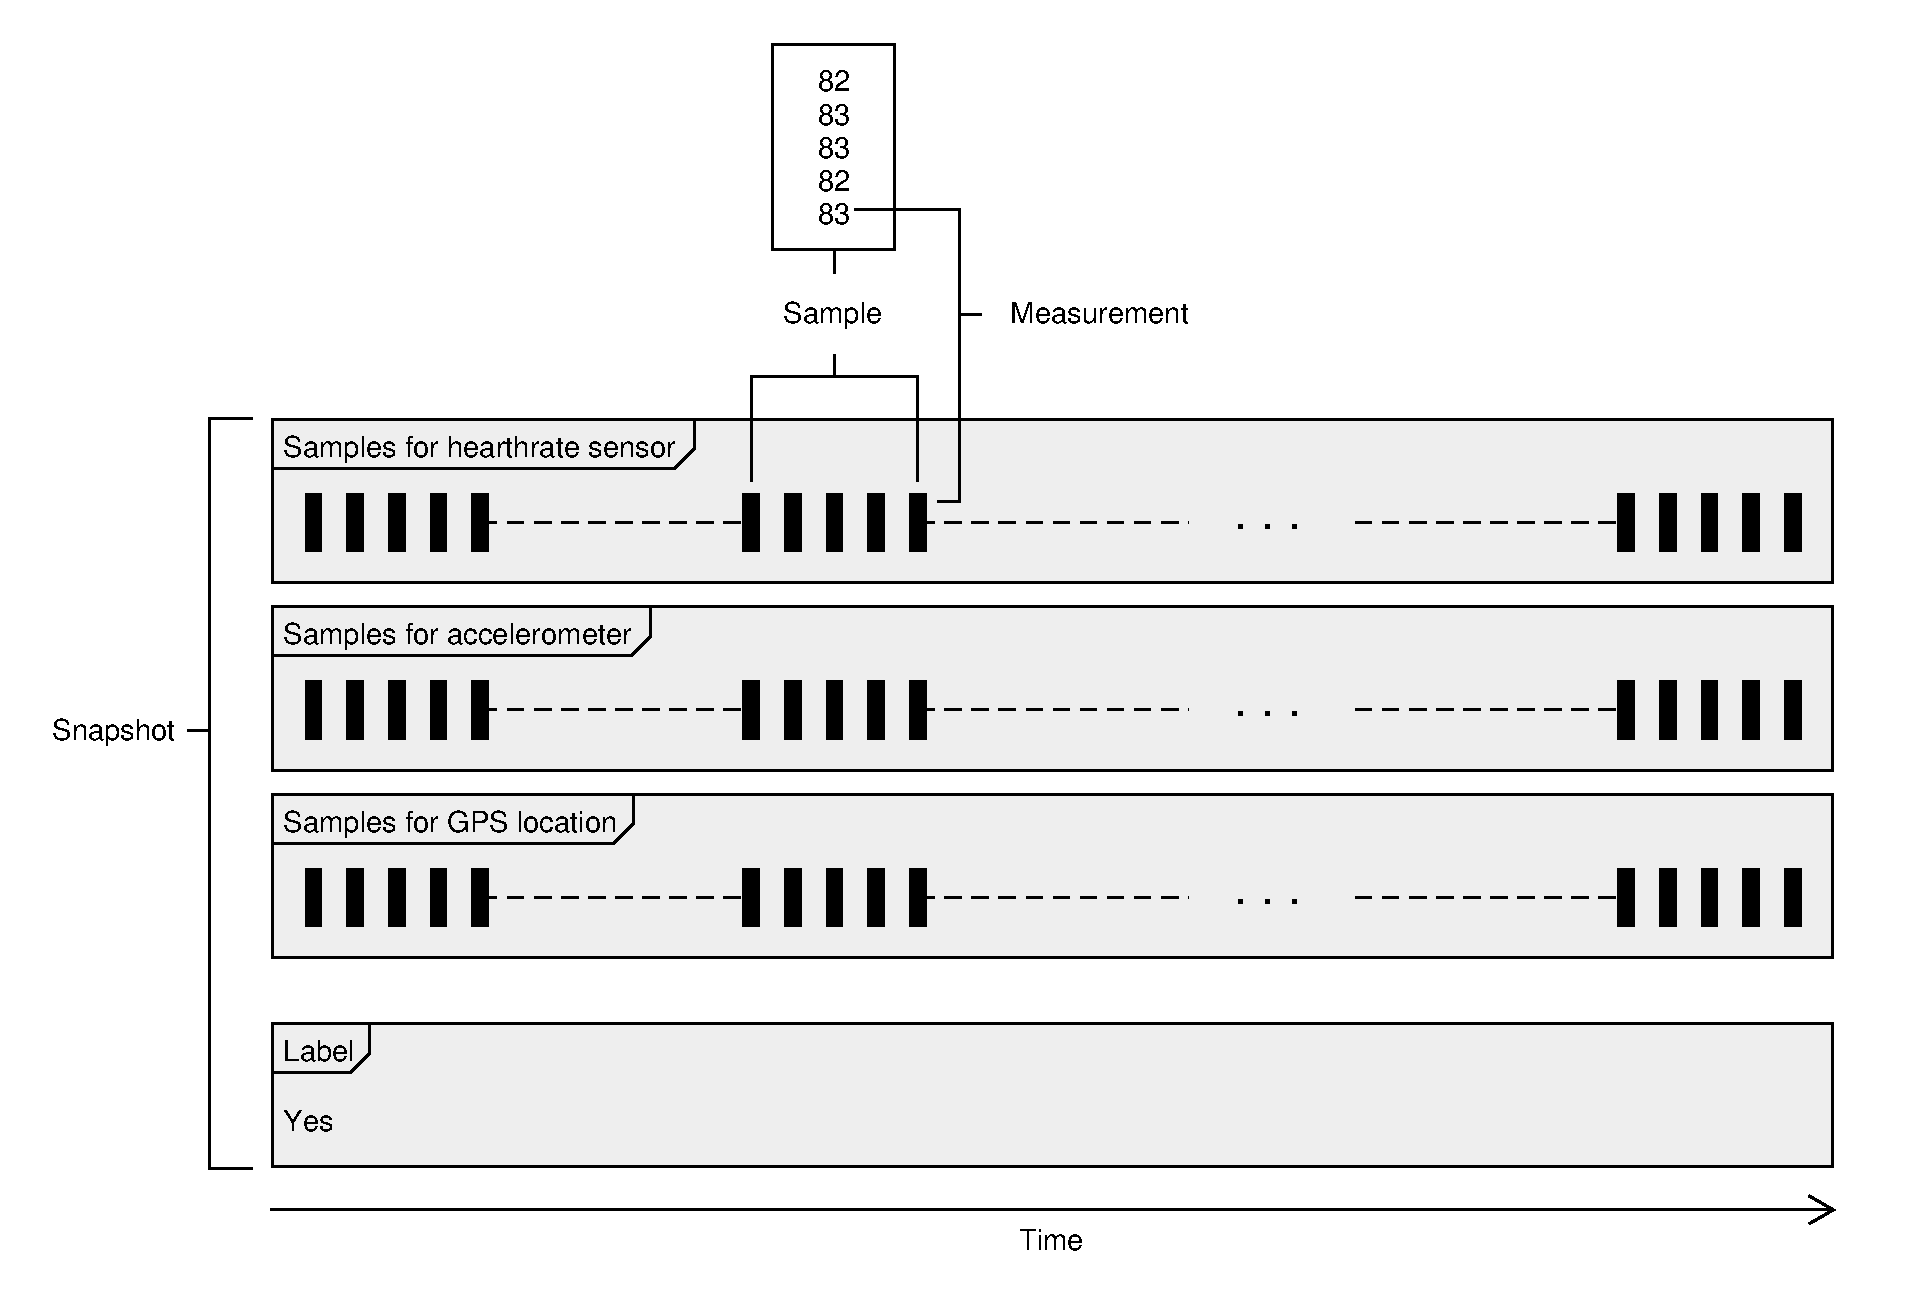
\includegraphics[width=\textwidth]{gathering_sensor_data/snapshot}
    \caption{Snapshot example containing measurements from three sensors and a label.}
    \label{fig:snapshot_example}
\end{figure}
\FloatBarrier

\todo[inline]{Beskriv hvad en campaign er i koden, brug gerne klassediagrammet til at forklare det!}

\begin{figure}[!htbp]
    \centering
    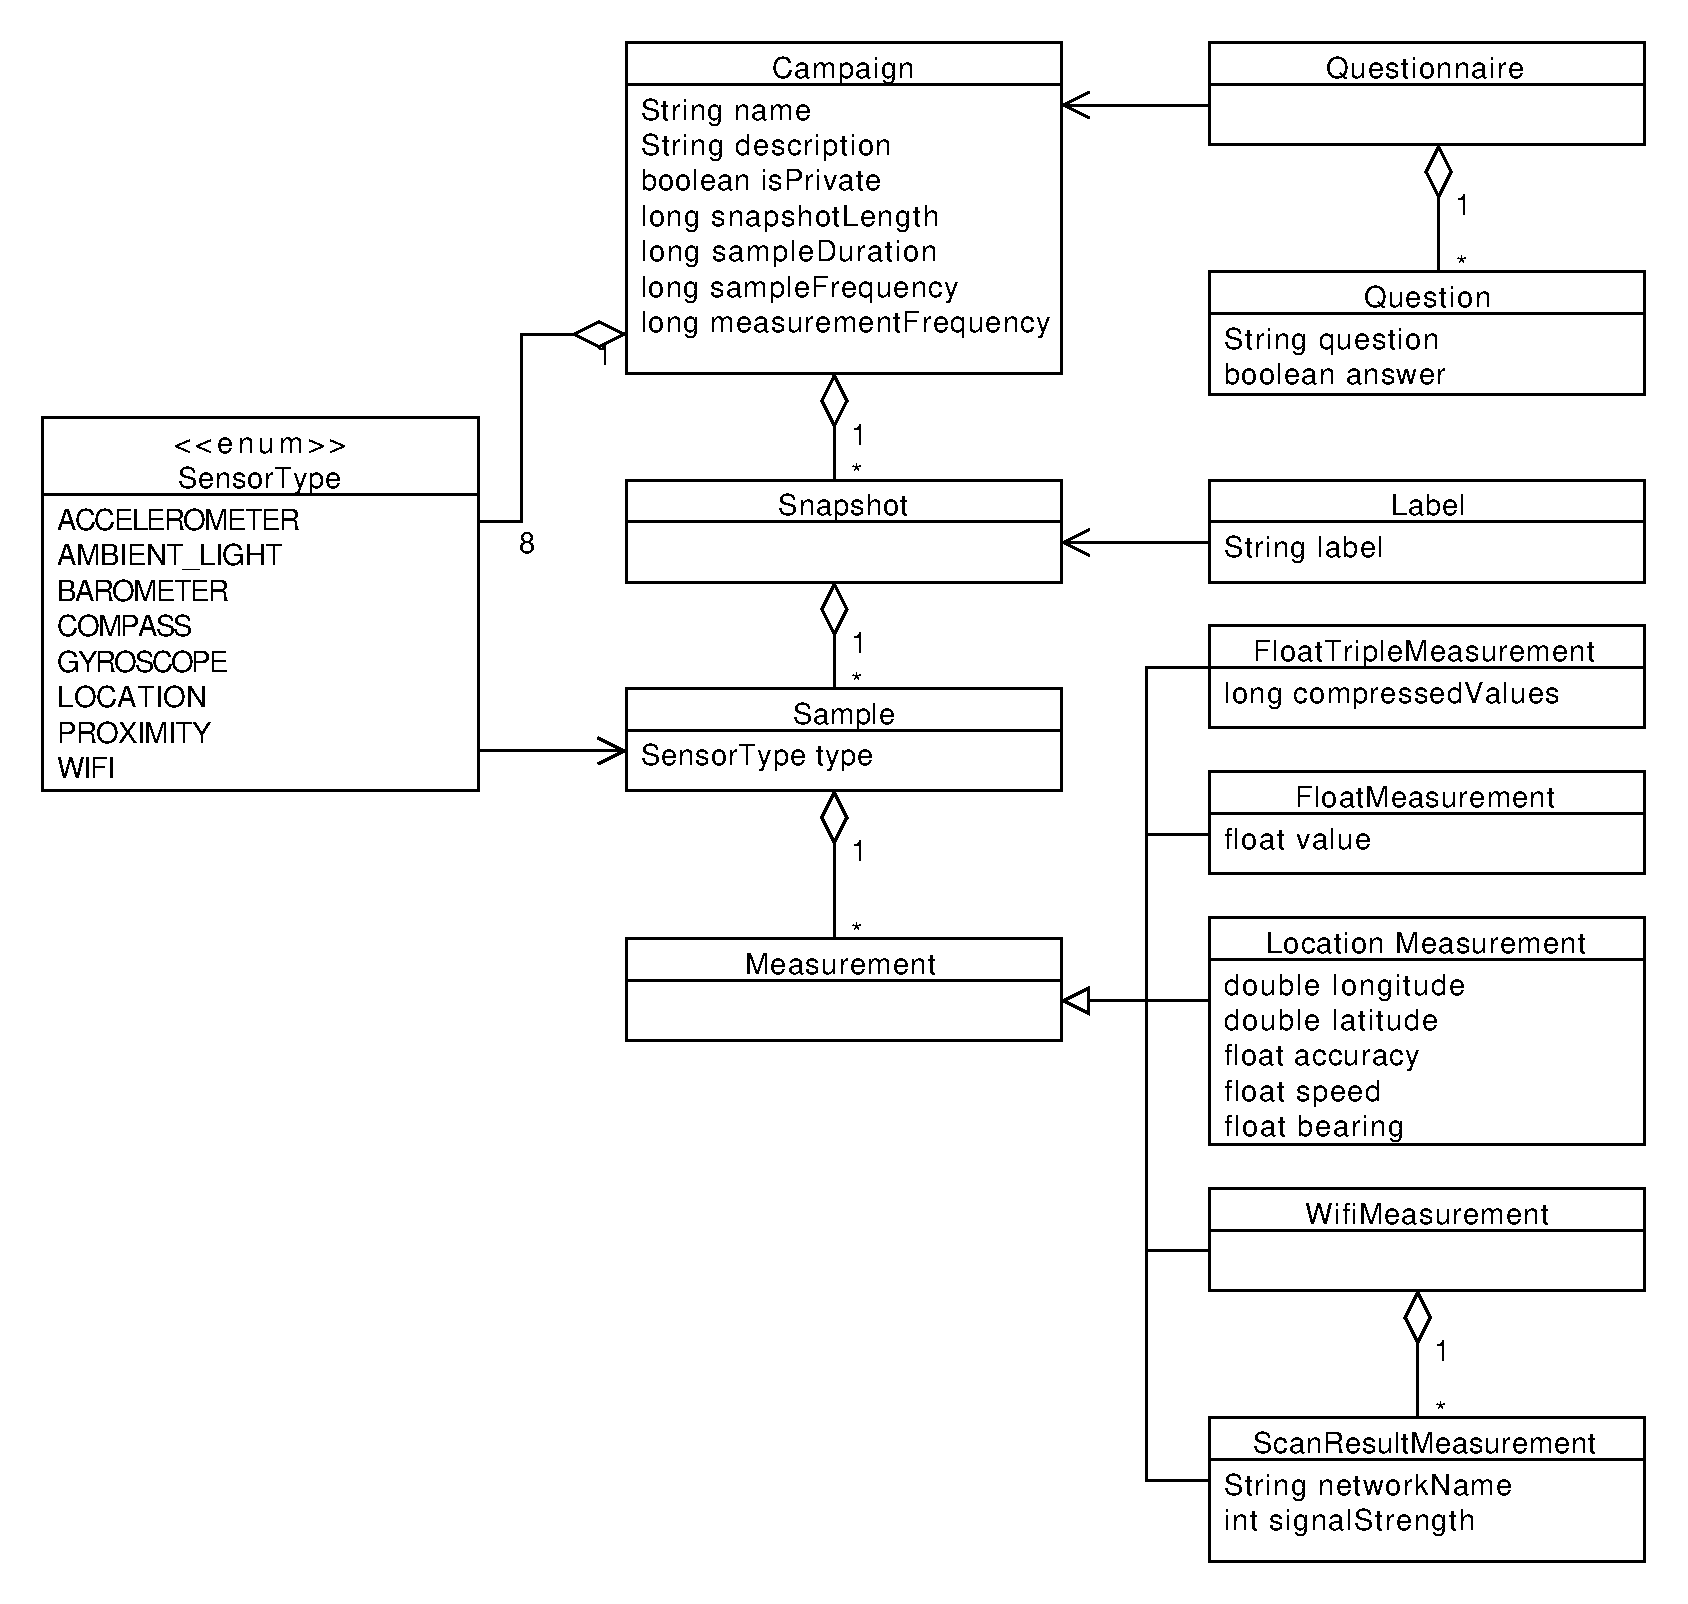
\includegraphics[width=\textwidth]{graphic/gathering_sensor_data/model_class_diagram.pdf}
    \caption{Class Diagram of the campaign model.}
    \label{fig:model_class_diagram}
\end{figure}
\FloatBarrier

\todo[inline]{ref til figur}

\subsection{Questionnaires}
We had come to the conclusion that customers should be able to define questionnaires to be a part of the data collection \secref{sec:human_activity_recognition}. Customers should be able to define one or more separate questions or more generally data inputs which combined should make out a questionnaire model. 
\\\\
Simple boolean yes/no questions can directly be combined to create a discrete amount of labels or classes which can later be used as targets for an AI model but more open inputs, which for instance can be used for regression or as more diverse features, should also be possible. \todo{Overvej om vi når at implementere continuous inputs}
\\\\
A questionnaire specification should be transformable to a format which can be easily be parsed and send from the server to the collecting devices. We have therefore implemented a questionnaire to be Java Parcelable. \todo{Overvej at ændre det her hvis vi gør det til JSON ting i stedet}



%!TEX root = ../../super_main.tex
\section{Structural Sensor Data}
\label{sec:structural_sensor_data}

Ideally we want to give the customers the ability to configure their campaigns completely in regards to what, i.e. which sensors should be included, and when the outputs from the sensors should be measured. This should be done in such a way that the customers can specify what data is important to them and still avoid draining the resources of the participants devices. For this reason we have designed a way to provide customers with the possibility to configure the temporality of their snapshots. 
\\\\
We go under the assumption that it will be possible to eaves drop in at all times meaning that we can retrieve a measurement from any sensor at all times, however this is not the case but this assumption is enforced as described in \secref{sec:providing_sensor_data}. With the axiom of the sensors we have structured the data from the sensors to be collected as shown in \figref{fig:sample_temporality}. In this figure we see the \emph{measurement} which corresponds to one reading or value of a sensor in a snapshot. Since a single \emph{measurement} from a continuous sensors does not make sense on their own, for instance a single measurement from accelerometer does describe the context in which the participants exist. We introduce a collection of such measurements which we call a \emph{sample}. A \emph{sample} is simply a stream of \emph{measurement}s where the interval or frequency (\emph{measurement frequency}) between them is configurable as seen in \figref{fig:sample_temporality}.

\begin{figure}[!htbp]
    \centering
    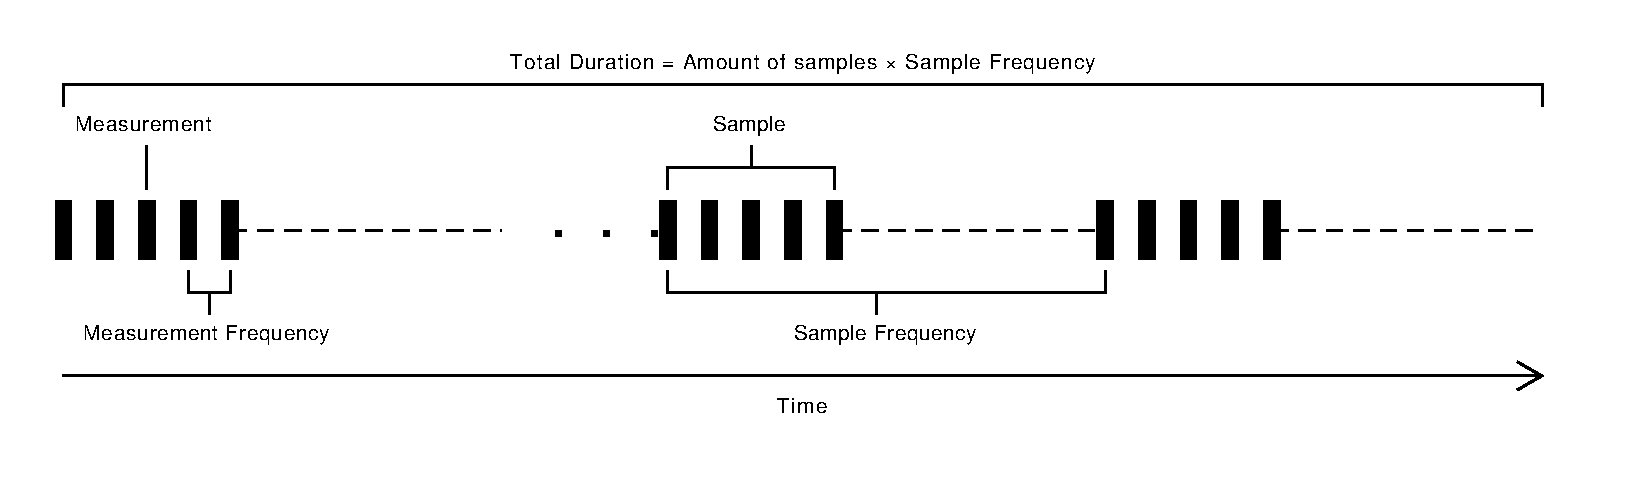
\includegraphics[width=\textwidth]{gathering_sensor_data/sample_temporality.pdf}
    \caption{Temporality of data for a single sensor in a snapshot.}
    \label{fig:sample_temporality}
\end{figure}
\FloatBarrier

Furthermore, we want the customer to configure how often these \emph{sample}s should be gathered, and for that reason we allow them to define a \emph{sample frequency}. And lastly the length of the of the snapshots is configurable by defining a \emph{total duration}, which states for how long the sensor should be measured in total.
\\\\
By this temporal structure of the sensor data we provide a viable way of configuring how the snapshots should be structured in regards to the sensor readings, while maintaining a uniform output format for customers of the system.

\todo[inline]{Vi har reelt 3 forskellige tider: Hvor længe skal et sample vare, hvor ofte skal vi tage et sample, hvor længe skal der gå imellem measurements i et sample? På grund af at sensore i Android giver svar når de har lyst, er det ikke sikkert at der kommer den samme mængde measurements i hver sample. Vi skal overveje om det giver mening, eller om det er vigtigere for kunden at hvert sample med garenti indeholder x measures. Problemet med dette er så at vi ikke kan sætte nogen garenti for hvornår disse measures reelt kommer.}

%!TEX root = ../../super_main.tex

\section{Providing Sensor Data}
\label{sec:providing_sensor_data}

To support this structure of the sensor output, we have designed an abstraction over the different sensors available. This abstraction is designed for concurrent collection of samples, as we want the application to be able to gather information from multiple sources at the same time, meaning that the system is able to, for instance, collect data regarding the motion and location of the participant simultaneously. This is done in order to make sure that the gathered data is obtained according to the desired temporality of the customer, i.e. the time constraints of the campaign.
\\\\
Problems will arise when enforcing temporality of snapshots due to the event oriented nature of sensors in Android. Sensor events will trigger whenever a value is updated. This effectively means that it is impossible to know when these events will trigger. We want to guarantee that measurements can be made with a specific frequency independent on what is supported by the sensor, i.e. measurements can be made more often than what some sensors provide, but also more rarely. To make it possible to always get samples at the desired rate, we need to store the last measured value. To do this, we will use a cache, containing the last measurement. This concept is illustrated on the message sequence diagram in \figref{fig:cached_values}. If multiple values are output from the sensors in between two sample readings, only the latest one will be considered by the sample collection unit. This might mean that some sensor readings will not be used for anything, but this is a necessary precaution we have to take, in order to ensure the temporal features of the snapshot. In the case where no measurements have been provided by the sensor, and the sample collector reads the cache, a default value will be read, which will reflect the fact that no measurements have been provided. It is then up to the customer to handle this.

\todo[inline]{Rikke: Need to explain the figure better}
\begin{figure}[!htbp]
    \centering
    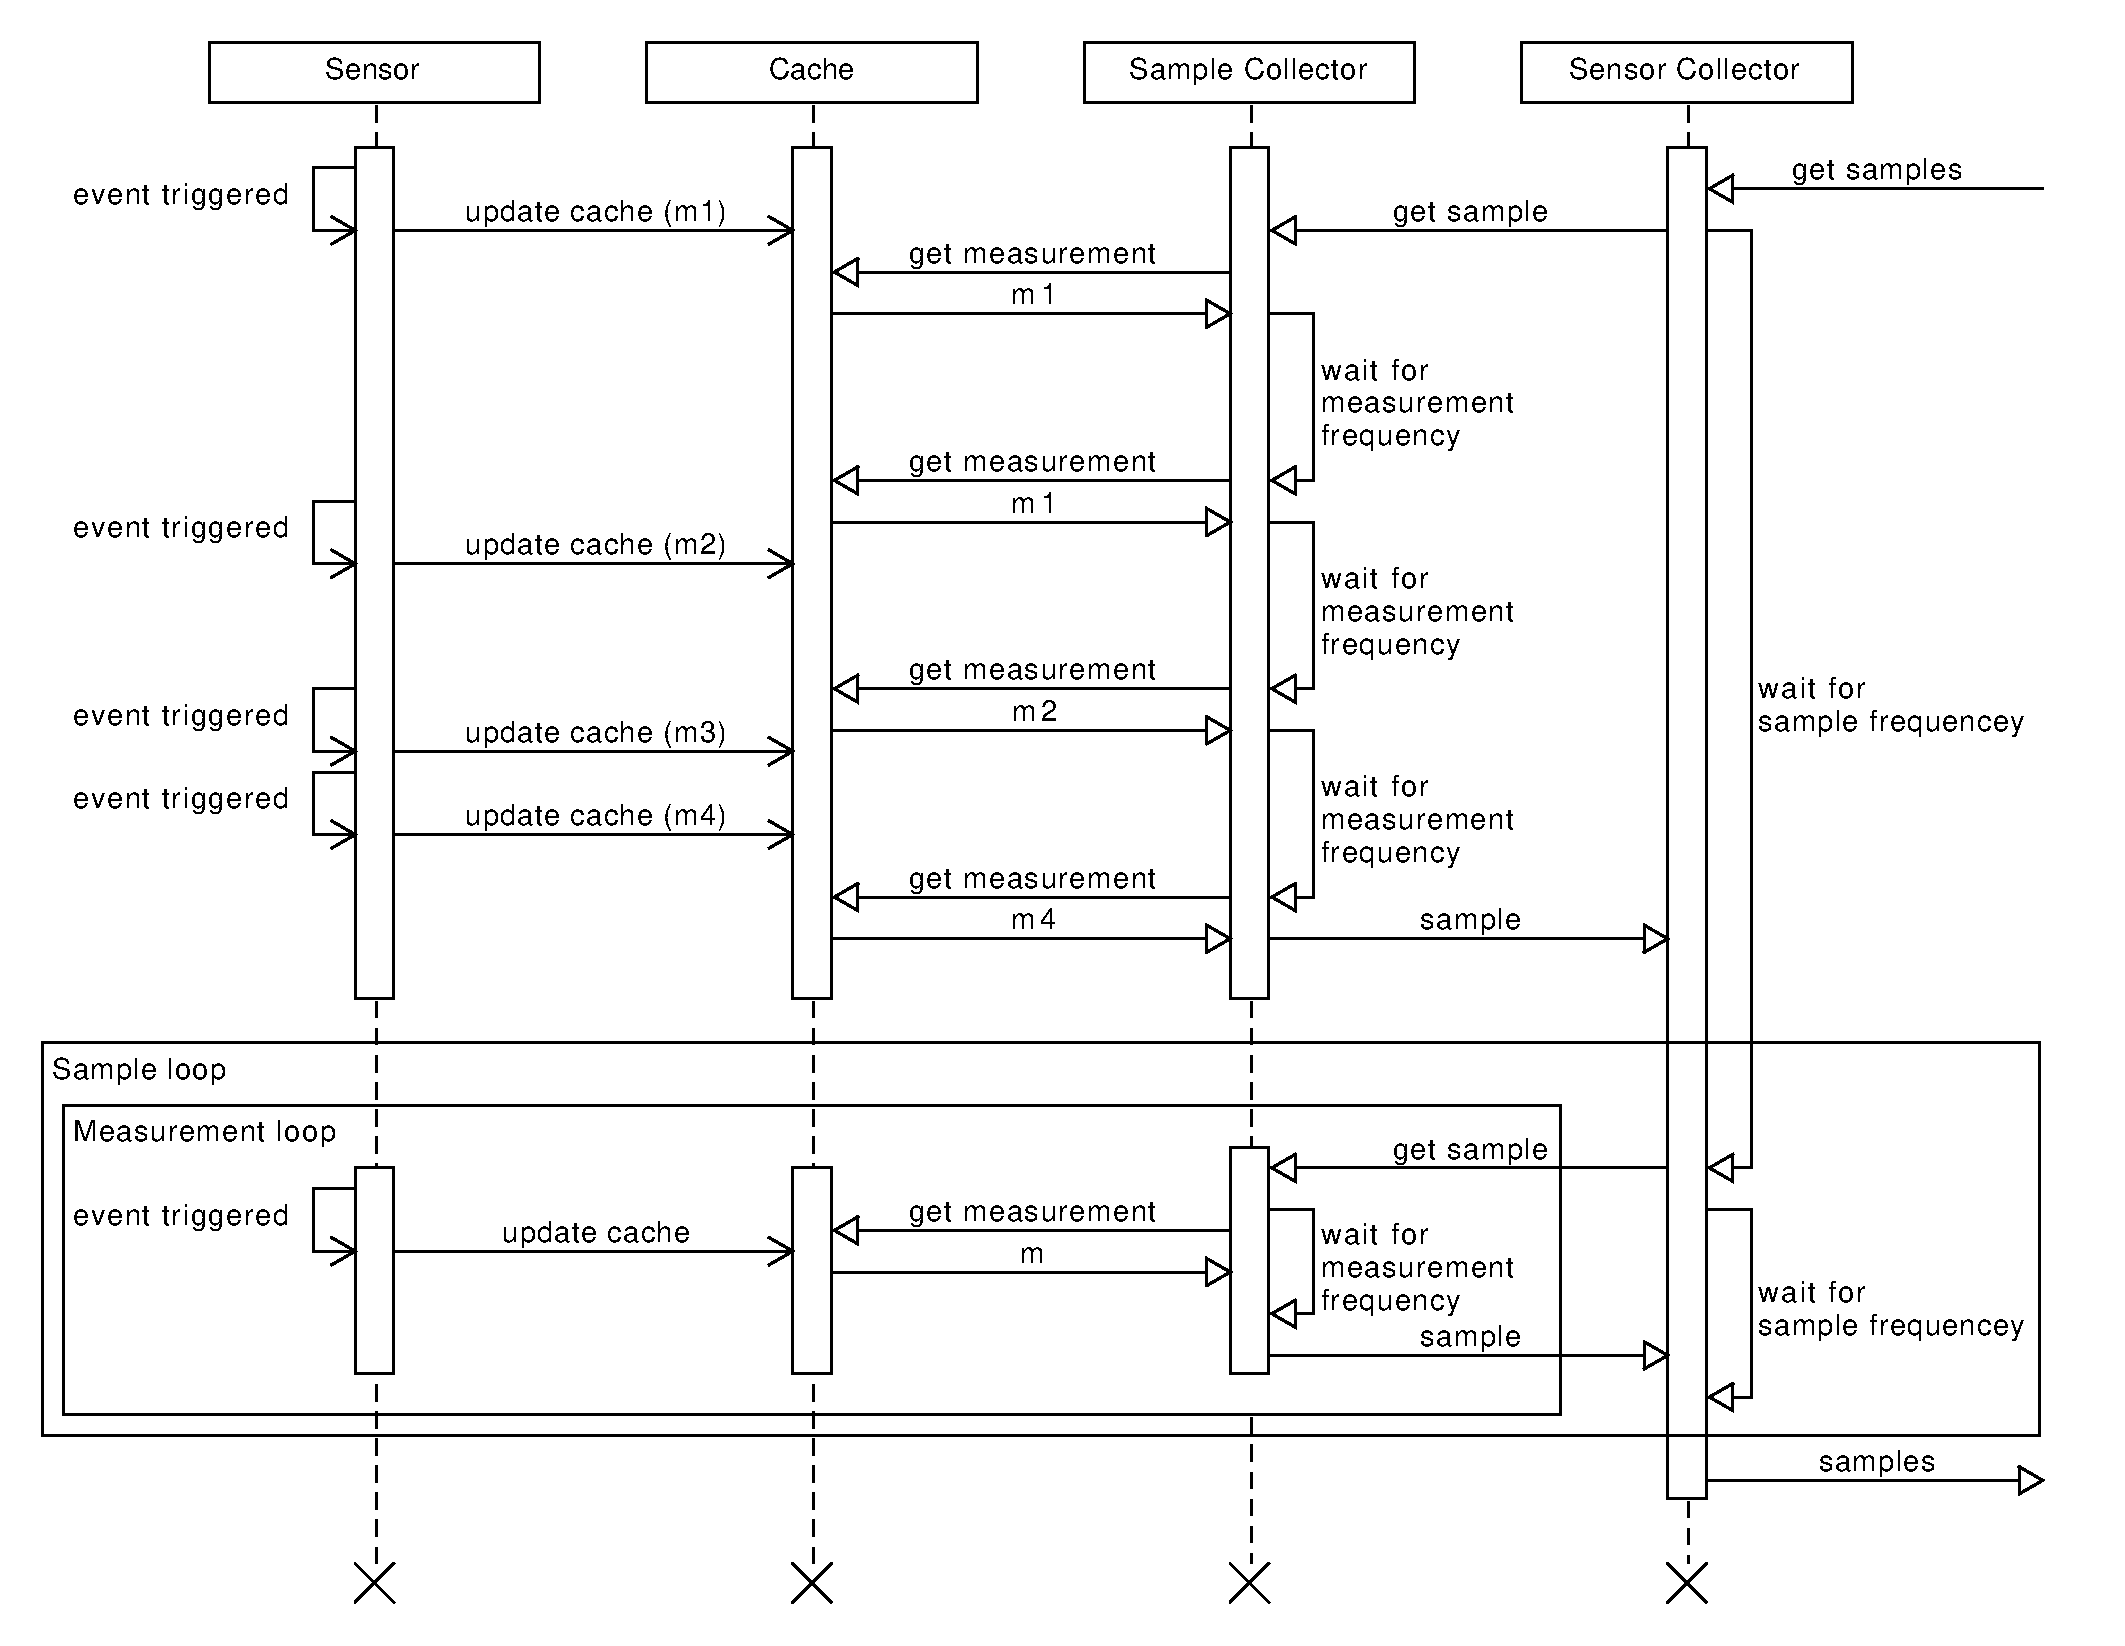
\includegraphics[width=\textwidth]{backgroundsensorservice/cached_values}
    \caption{Snapshot creation based on cache to ensure desired temporality.}
    \label{fig:cached_values}
\end{figure}
\FloatBarrier

\subsection{Implementation}
\label{sub:providing_sensor_data_implementation}
We have implemented an abstract class called \mono{SensorProvider}, which must be specialized for each type of sensor available, both for sensors found in Android, but also for sensors found in the Microsoft Band 2. The abstract class provides functionality that makes it easy to implement specialized implementations for every sensor that we have. Sub-classes of the abstract \mono{SensorProider}, must specify a generic argument, \mono{MeasurementT}, describing the type of measurement that the implementation will make. Besides this, the following methods must also be implemented on the specializations:

% The common interface for these sensor providers is implemented by the following methods:

\begin{description}
	\item[\mono{boolean isSensorAvailable()}] Should return \mono{true} if the sensor is currently available, and ready to take measurements. Should return \mono{false} if the sensor is unavailable or not present on the device.

	\item[\mono{SensorType getSensorType()}] Should return the \mono{SensorType} that the sensor provider implementation will utilize. For instance \mono{SensorType.BAROMETER}.

	\item[\mono{EventListenerRegistrationManager createRegManager()}] Should return an instance of something that implements the \mono{EventListenerRegistrationManager} interface. This interface will enforce the class to implement the following two methods: \mono{void register(int frequency)} and \mono{void unregister()}. These methods will be used by the \mono{SensorProvider} implementation to register the sensor (and its event listeners) when the specific sensor is needed, and unregister them when they are not.
\end{description}

Besides implementing these methods, the specializations must also call the \mono{void onNewMeasurement(MeasurementT)}, which will override the cached value, as preciously described in \figref{fig:cached_values}. With these measurements registered, the \mono{SensorProvider}, and in effect all of the sub-classes, are now able to construct \mono{Sample} objects by reading measurements from the cache with the specific intervals. 
\\\\
All of this effectively means that new sensors can be implemented into the system with very few lines of code. An example of such an implementation can be seen in \lstref{lst:sensor_provider_acclerometer}, which shows how the \mono{AccelerometerSensorProvider} implements and uses the methods described above to make measurements from the phones accelerometer available to our application. 

\todo[inline]{Rikke: Need to explain the code better}
\lstinputlisting[
   style = Java,
   caption = {Implementation of sensor provider for Accelerometer.},
   label = {lst:sensor_provider_acclerometer},
   float,
]{content/gathering_sensor_data/code_snippets/sensor_provider_acclerometer.java}

% The abstract \mono{isSensorAvailable()} method allows the subclasses of \mono{SensorProvider} a way of specifically checking if the device has that sensor available. This might for example be useful in order to determine which campaigns should be available to which participants at some point, or detecting if a wearable device has been disconnected. \mono{retrieveSampleForDuration()} is a method that every subclass has to implement, which specifies how a sample is created for this specific sensor. The \mono{retrieveSamplesForDuration()} method is implemented on the \mono{SensorProvider} class, i.e. not abstract like the other two methods, and is the method that makes all the different providers work asynchronously. The method returns a \mono{Future<List<Sample>{}>}. A future, in Android, is the result of an asynchronous computation. The result from a future can be retrieved by calling the \mono{get()} method on the future object, which is a blocking call. Android then provides different methods to check whether or not the computation is completed, in progress, and so on. The method works by submitting a \mono{Callable} to a thread pool, which will eventually return a list of samples, i.e. the future. This callable contains a \mono{TimerTask}, which is a task that is repeated a certain amount of times, that in return calls the \mono{retrieveSampleForDuration()} method. In that way, we have a \mono{Callable} which at some point returns the desired amount of samples. 
% \\\\
% The \mono{retrieveSampleForDuration()} method has, in all the subclasses of \mono{SensorProvider}, been implemented by using a native method called \mono{onSensorChanged()}. As the name implies, this event is triggered whenever a sensor changes its state. This is a potential issue, since not all sensors provide continuous data, and not all sensors will change in the time limit that is allowed between two measurements (see \figref{fig:sample_temporality}). A potential solution to this is to always store the previous state, and if the event is not triggered within the alloted time, simply use the cached value. 
% \\\\
% Another potential issue with this implementation is the desire for asynchronism, which we implemented by using \mono{future} objects. Since we cannot know for certain when different asynchronous calls are finished, it might become difficult to create a snapshot and send it to the database.

% \lstinputlisting[
%    style = java,
%    caption = {Property similarity on a component.},
%    label = {lst:attribute_difference},
%    float,
%]{content/implementation/annotation/attribute_difference.java}

%!TEX root = ../../super_main.tex

\section{Background Sensor Service}
\label{sec:background_sensor_service}

We have implemented a service, which we call Background Sensor Service, in order to facility non-intrusive data collection in the Android system.
This section includes some technical details about how services work in Android and how we have implemented our Background Sensor Service. 

\subsection{What is an Android service?}

A services in Android is an application component which encapsulates long running background processing or a way to provide access to a shared ressource. Services can be shared and can be configured run independently, i.e. running in a different process, from the graphical interface shown to users, which is ideal for our background data collection. Services have their own lifecycles and can be configured in many different ways. They can be configured as an API where the service itself has a short lifespan while serving some data or while performing a short task or they can be configured as a long running background task with its own complex behavior.
\\\\
% Message parsing
The Android framework supports two-way message parsing as a way of communication with a service when it runs in a different process. Message parsing makes it easy for the Android \mono{Activity} elements in the graphical and interactive part of the application to communicate with our Background Sensor Service.
\\\\
We have given an overview of the concurrency 

\subsection{Service Start}

% Boot receiver
% On Application start
Our Background Sensor Service should ideally always be running, which does not imply that it is constantly using processing ressources. We have implemented two measures to ensures that the service is running for as much time as possible. We have implemented an Android BroadcastReceiver, which upon receiving a system wide boot completed action (\mono{ACTION\_BOOT\_COMPLETED}), starts the service. The service is also attempted started everytime the application is started, but is not started twice if the service is already running. 

\subsection{Snapshot Generation and Synchronization}
\label{sub:background_sensor_service_snapshot_generation_and_synchronization}

The background Background Sensor Service uses two independent timers. One for Snapshot generation and one for synchronization of the snapshots with our server. The timer for snapshot generation is encapsulated in a class called \mono{SnapshotTimer} which is started whenever the service has an active running campaign which should generate snapshots. Timed tasks are then scheduled at a constant rate, generating snapshots, until the campaign is completed or stopped by the user.
\\\\
Synchronization of snapshots with the server is done with the second timer which is encapsulated in a class called \mono{SynchronizationTimer}. \mono{SynchronizationTimer} schedules tasks, when active, which attempts to synchronize gathered snapshots with the server at a fixed rate if the device is currently connected to a WiFi network. This is not an optimal solution as it does not incorporate any battery consumption optimizations except maybe for a little bundling of the data in the given temporal frame until the next synchronization. The actual size of the bundled data is not taken into account so the bundling of the collected data is probably not that effective, especially not for data sets collected at a low frequency. The \mono{SynchronizationTimer} also does not incorporate any radio based optimizations such as scheduling network task through Android APIs. The \mono{SynchronizationTimer} just requests immediate communication over the WiFi connection which forces waking up radio hardware if it was in a dormant state. This is not ideal as we do not require data to be uploaded as soon as its ready as stated in \todo{Byg ref til vores opsummering af krav jf. task til at gøre det} and because there is potential for less battery consumption which would help satisfy \todo{ref til konkret requirement }. 
\\\\
An example of an Android API, or rather a library with Google APIs for Android, which could help optimize network usage would be the \mono{GCMNetworkManager} class, which is an Android service, that can schedule encapsulated network tasks. \mono{GCMNetworkManager} \parencite{gcmnetworkmanager} handles batching of network tasks; retries; backoffs, in case a remote server is not responding or is busy; waiting for WiFi, for bandwidth heavy communication; waiting with commutation until the device is charging; and waiting until a radio becomes active, for instance by getting activated by another application. It does all of this based on parameters given to every encapsulated network tasks such as a desired time frame for the network communication and desired network or battery conditions.  
\\\\
Adding such optimizations should however be doable as all data synchronization work is local to the \mono{SynchronizationTimer} and not distributed elsewhere in the implementation. Other network tasks such a refreshing GUI with lists of Campaigns from the service should happen instantly and are thus more difficult to optimize. 

\subsection{Background Sensor Listening}

The Background Sensor Service is configured to have one thread, in a pool of threads, available per sensor type, i.e. per \mono{SensorProvider}, see \secref{sub:providing_sensor_data_implementation}, instance used in the service. This lets the scheduling of the gathering from the different \mono{SensorProvider} instances up to the underlying Java implementation of threads in a hope to run the different types of sensors and other data sources as independently as possible. Data is only collected from the \mono{SensorProvider} instances if the corresponding sensors are included in the currently active campaign and if the system is currently gathering a snapshot. There is no data collection activity in the Background Sensor Service unless a timed task for a snapshot is running. CPU resources and thereby battery is therefore only consumed on demand.
\\\\
We do not provide any real time guarantees but the different threads from the different streams of data should always be able to run unless they get starved by other processes in the system. Temporary starvation of the data collecting threads might result in missed updates from different data sources. 

\subsection{Concurrency Overview}

We have attempted to give an overview of the current processes and threads running in the mobile application in \figref{fig:system_currency_and_lifecycle} illustrated with a near UML Activity Diagram Syntax. 

\begin{figure}[!htbp]
    \centering
    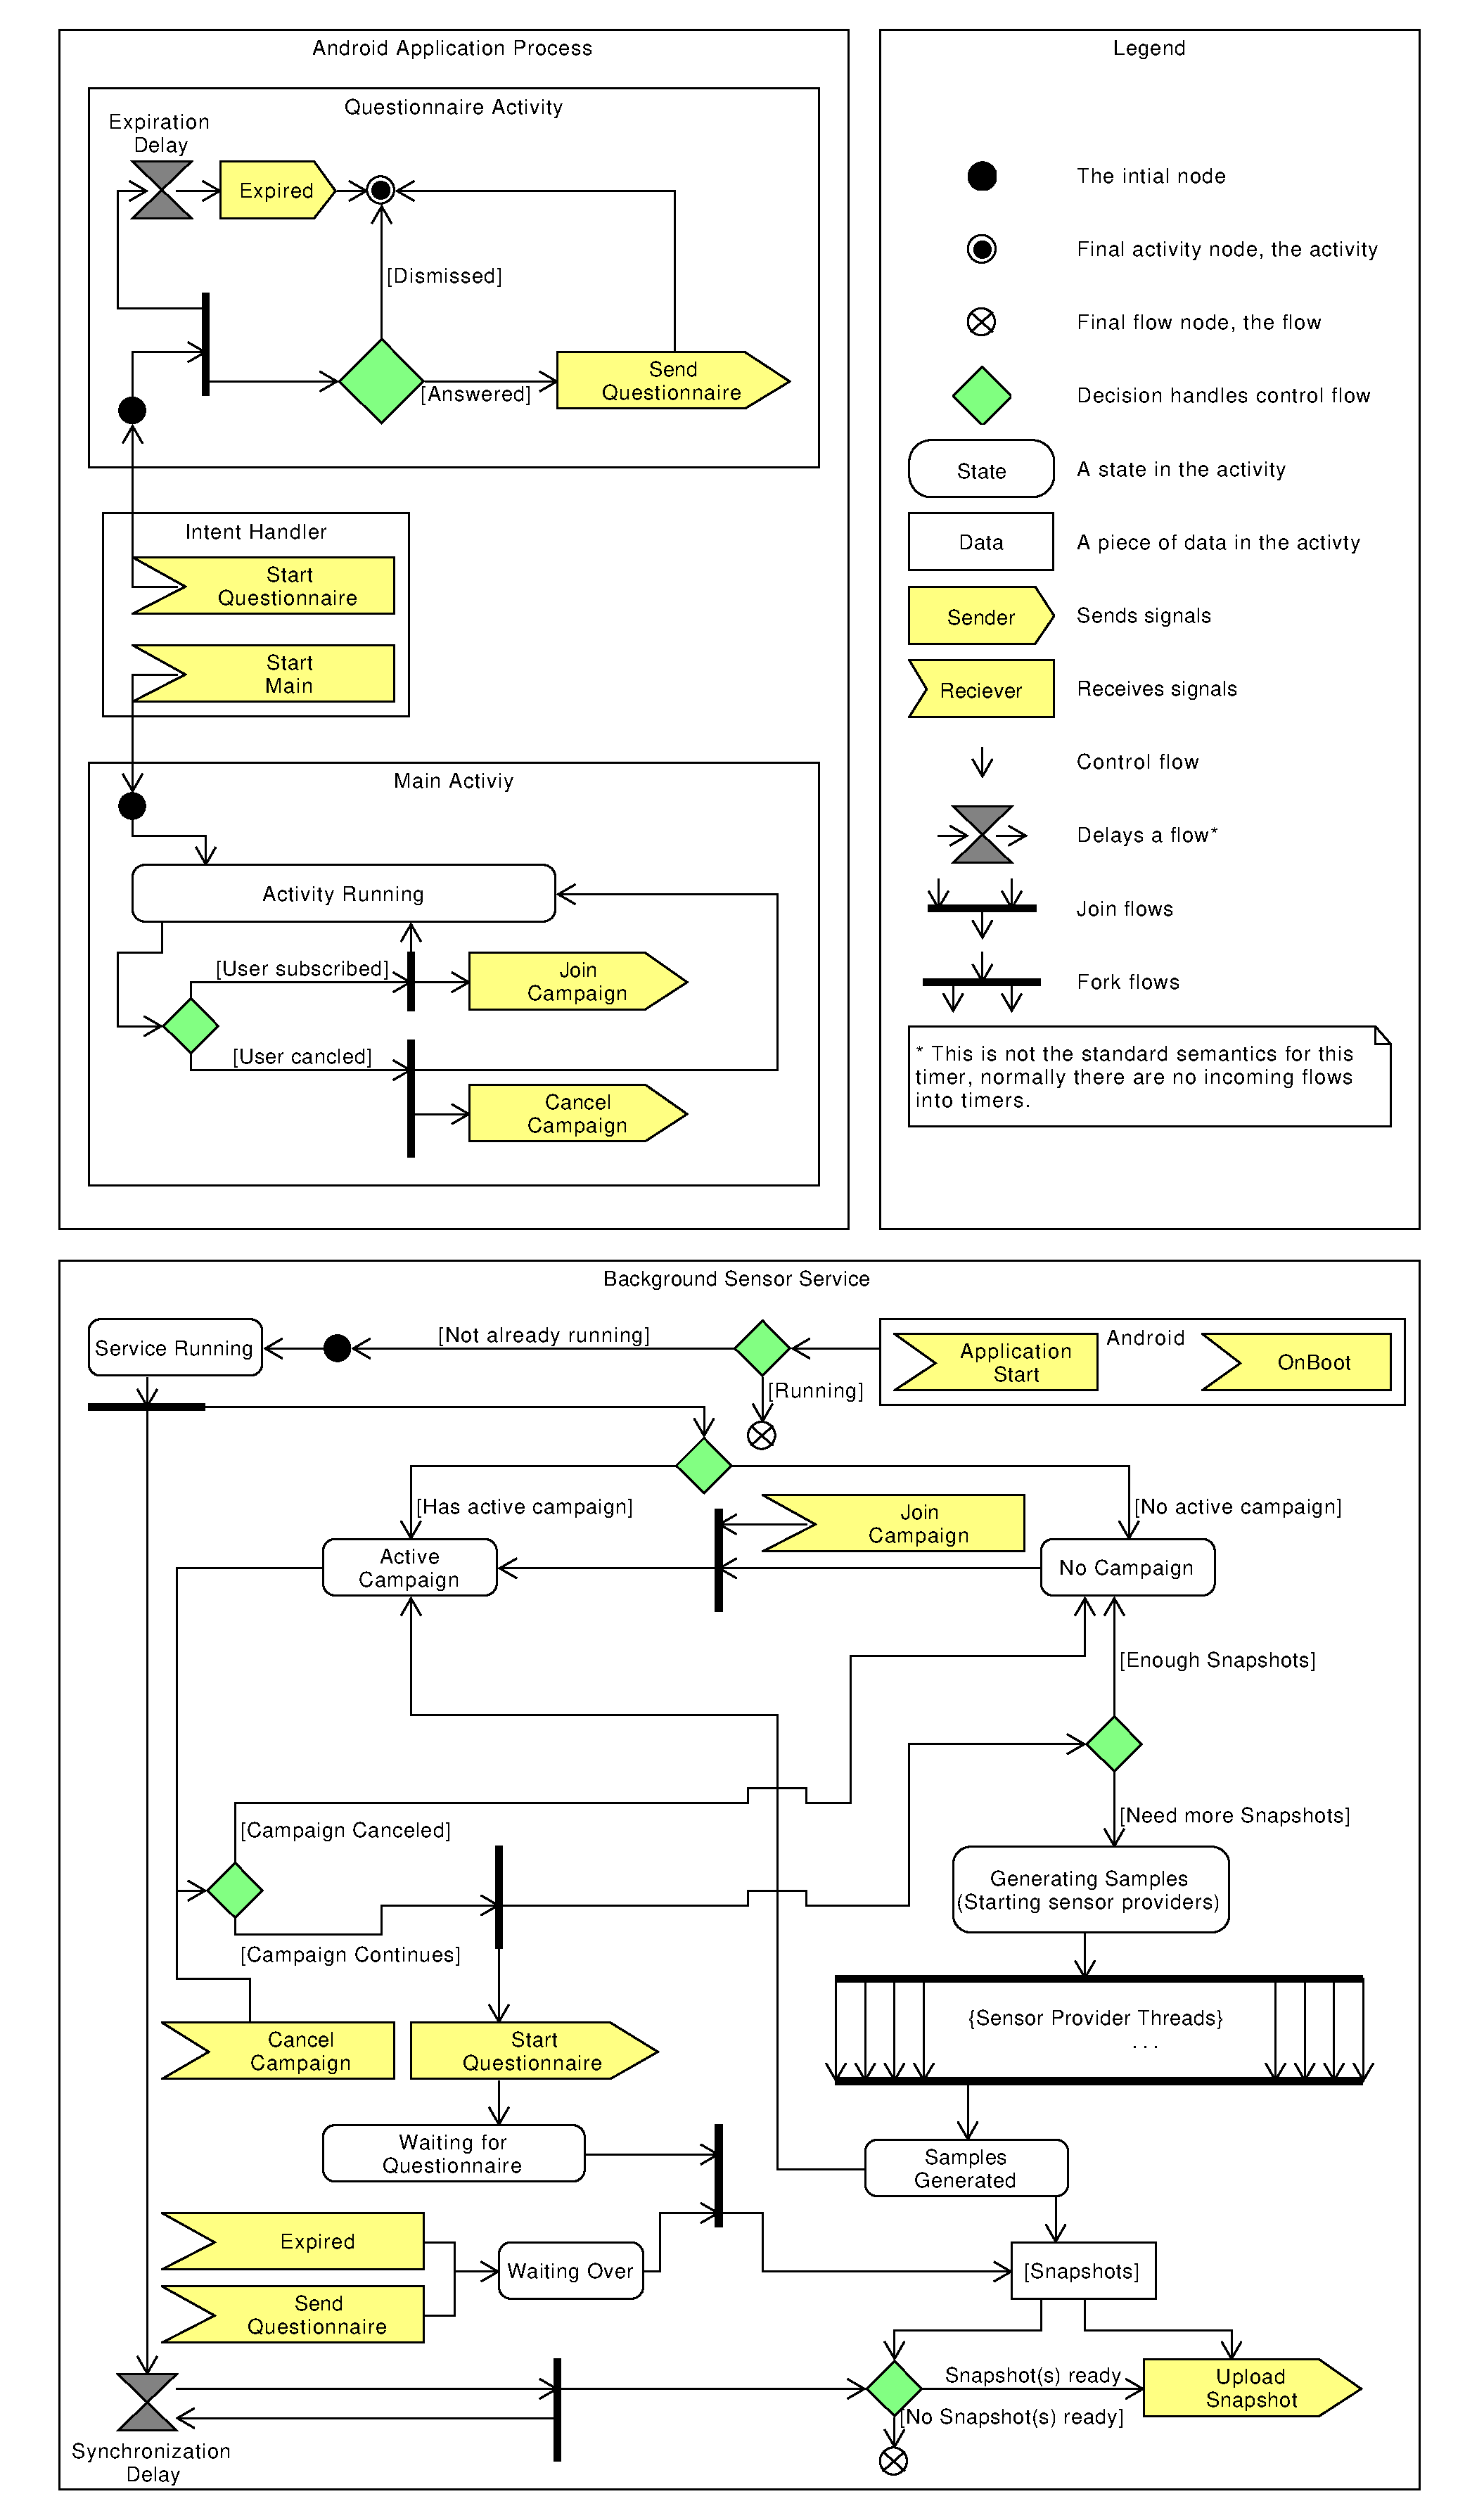
\includegraphics[width=\textwidth]{graphic/backgroundsensorservice/lifecyclestuff.pdf}
    \caption{An Activiy Diagram like overview of the mobile Application Components.}
    \label{fig:system_currency_and_lifecycle}
\end{figure}
\FloatBarrier

%!TEX root = ../../super_main.tex

\subsection{Data Quantity Estimation}
\label{sec:data_quantity_estimation}
%This gave us a dataset with a size of 142908 bytes. This experiment would then yield a data set of approximately 205 MB if it was run for a day. Running the same experiment for 30 days with 100 different devices would then approximately yield a data set of 617 GB assuming similar mobile devices with similar sensors. This quick napkin math was only for one sensor with 100 people and this could quickly escalate if more sensor or more people are added.

\todo[inline]{Overvej: Lav en reference til vores user story, og fortæl hvor meget data vi samler om dagen med disse målinger. Skriv også at dette KUN er RÅ sensor output, stored i Java-hukommelse størrelser. Med snapshot struktur er det meget værre} 

According to our problem statement in \secref{sub:problem_statement}, we want to minimize the effect that our application has on the  daily mobile lives of participants. One aspect that might have influence on this is the battery consumption and network usage of our application. We would there like to minimize these factors. In order to do this, we have experimented with different continuous sensors on a Nexus 5 smartphone and logged all values captured from the sensor for 1, 5, and 20 minutes. The results of these tests can be seen in \tabref{tab:sensor_experiment}. Note that the orientation sensor is a virtual sensor, which uses data collected from both the gyroscope and magnetometer, hence the correlation between the data sizes ($143 \text{KB} + 35 \text{KB} \approx 177 \text{KB}$ for 1 minute). These tests were only performed for four different sensors, but customers might need data from several different sensors, thus further increasing the amount of data collected. These quantities of data might present a problem even on modern mobile platforms due to paid limited data plans and battery consumption. There might be different data needs, some customers might require very detailed data from many sensors from a few devices and others might require more sparse data from a few sensors from a lot of different devices. However, we can conclude that gathering a continuous stream of data from all sensors all the time is not a viable solution.

\begin{table}[!htbp]
\centering
\begin{tabular}{l|c|c|c|c}
\textbf{Sensor}     & \textbf{Accellerometer} & \textbf{Gyroscope} & \textbf{Magnetometer} & \textbf{Orientation} \\ \hline
\textbf{1 minute}   & 142 KB                  & 143 KB             & 35 KB                 & 177 KB               \\ \hline
\textbf{5 minutes}  & 714 KB                  & 714 KB             & 178 KB                & 892 KB               \\ \hline
\textbf{20 minutes} & 2,859 KB                & 2,859 KB           & 715 KB                & 3,573 KB                
\end{tabular}
\caption{Data size of sensor data collection after a set amount of time.}
\label{tab:sensor_experiment}
\end{table}
\FloatBarrier

%!TEX root = ../../super_main.tex

\section{Compression}
\label{sec:compression}

As described in \secref{sec:data_quantity_estimation}, we would like keep the power consumption of our application low. One way of doing this is ensuring that the amount of data sent from our application to our server is the minimum amount necessary, because sending less data costs less power. During the development we discovered that many of the data types used for sensor measurements have significant overhead, compared to what is necessary in order to store the data, which opens up for the possibility of compressing the data. 
\\\\
An example of this is the heart rate sensor in the Microsoft Band 2 wearable, which uses an signed integer in order to store a heart rate. A signed integer is typically 32 bits, and has a maximum value of $2^{31} - 1$ (2,147,483,647), while a heart rate over 250 is very abnormal. This knowledge would allow us to exploit the limited value range, and use as little as 8-10 bits (values 255-1023). This would effectively cut off the majority of bits used to store a value. Furthermore, Microsoft Band 2 also uses a boolean to represent if the reading is precise (they call it locked), which uses 8 bits. This effectively means that even if you use 10 bits for the heart rate, and 1 for the locked state, you would still save 29 bits.    
\\\\
There are many more cases like that in the sensor readings, and we decided to implement a strategy for compressing one of the common values returned by many sensors, namely an array of floats containing three values. An example of a sensor that returns such measurements is the accelerometer which measures how the phone moves on its $x$, $y$, and $z$ axes. We designed a class called \mono{FloatTripleMeasurement} which is used to compress these three values to a single \mono{long}, meaning we convert $12$ bytes ($3$ floats $\times 4$ bytes) to be stored in $8$ bytes. We do this by sacrificing some of the precision of a regular float, because we think the regular precision is overkill, both in terms of sensor inaccuracy and also its usefulness for the customers. When compressing, we assume that the integer part (of the float) does not exceed $7$ numbers. We do this because the sensors only produce values ranging from $-360$ to $360$. We strip the decimal separator from the floats and treat them as a $20$ bit integer value, where the first bit determines whether the value is positive or negative. This means that we now use $60$ bits for storing the compressed value of the floats. We use the remainder of the long to add 3 bits for representing where the decimal should be placed. A visualization of the method used to compress floats can be seen in \figref{fig:float_triple_convert} and \figref{fig:float_triple_bit} respectively.

\begin{figure}[!htbp]
    \begin{alignat*}{6}
       &8.138   &&                   &&   && 8138  &&                   && \text{\mono{00000001111111001010}} \\
      -&12.821  && ~~ \rightarrow ~~ && - && 12821 && ~~ \rightarrow ~~ && \text{\mono{10000011001000010101}} \\
       &42.4878 &&                   &&   && 42487 &&                   && \text{\mono{00001010010111110111}} 
    \end{alignat*}
    \caption{Compression of floats.}
    \label{fig:float_triple_convert}
\end{figure}
\FloatBarrier

\begin{figure}[!htbp]
    \centering
    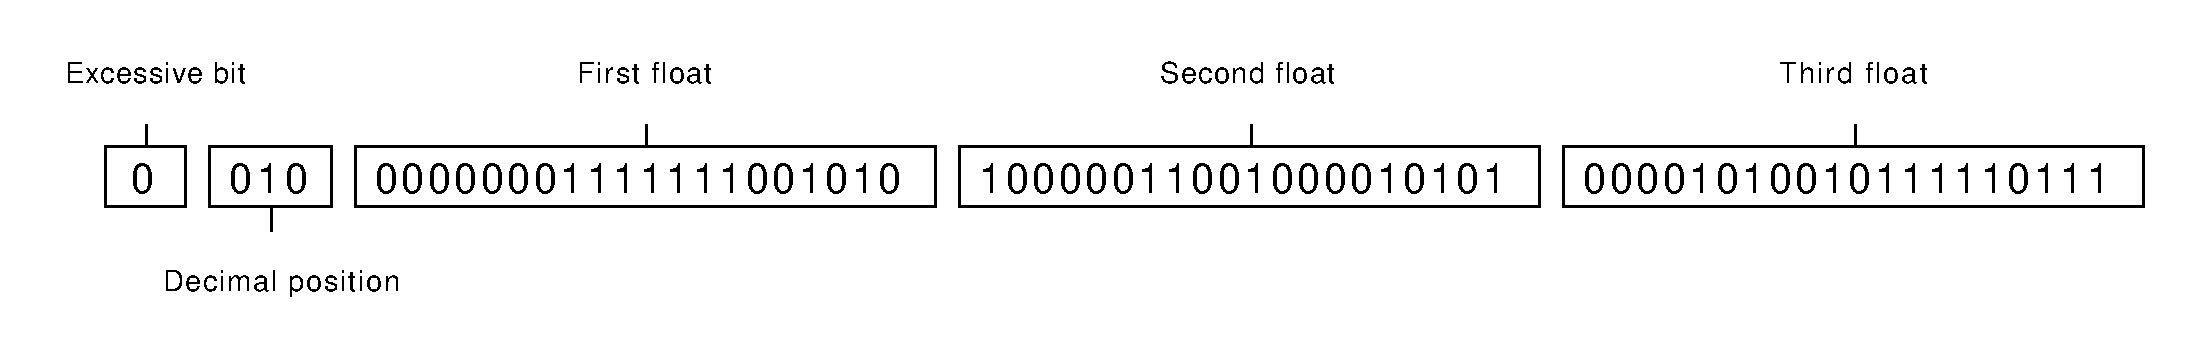
\includegraphics[width=\textwidth]{graphic/gathering_sensor_data/float_triple_bit}
    \caption{The bit representation of a \mono{FloatTripleMeasurement}.}
    \label{fig:float_triple_bit}
\end{figure}
\FloatBarrier

We wanted to compress the floating point values of the sensors so that the size of the data we need to send over network and store on the device would decrease. However, this compression does not come for free. We actively make a trade off between size of data stored and CPU cycles used for compressing and decompressing the values. We have conducted a performance test for our compression of floats that investigates how much extra time has to be spent on compressing and decompressing the floats. In the test we create a number of arrays that each contain three float values. The actual test is how fast the three float values can be multiplied together. We do this in two ways: One where we compress and decompress the float values first, and another one where we just multiply. This can give us an indication of how much time is lost on the compression when performing another task. The results of the test can be seen in \tabref{tab:results_of_compression_test}.

\begin{table}[!htbp]
\centering
    \resizebox{\textwidth}{!}{%
        \begin{tabular}{|l|l|l|l|l|l|l|}
            \hline
            ~ & \multicolumn{3}{|c|}{1+ One} & \multicolumn{3}{|c|}{Nexus 5 } \\ \hline
            Count    & \begin{tabular}[c]{@{}l@{}}With \\ compression\end{tabular}  & \begin{tabular}[c]{@{}l@{}}Without\\ compression\end{tabular} & Ratio & \begin{tabular}[c]{@{}l@{}}With \\ compression\end{tabular}   & \begin{tabular}[c]{@{}l@{}}Without \\ compression\end{tabular} & Ratio \\ \hline
            10000   &   83 ms   &   11 ms   & 7.55  &   77 ms   &   10 ms   & 7,70  \\ \hline
            100000  &  635 ms   &  172 ms   & 3.69  &  783 ms   &  113 ms   & 6,93  \\ \hline
            1000000 & 9088 ms   & 1333 ms   & 6.82  & 8245 ms   & 1090 ms   & 7,56  \\ \hline
        \end{tabular}%
    }
    \caption{Results of compression test}
    \label{tab:results_of_compression_test}
\end{table}
\FloatBarrier

As can be seen in \tabref{tab:results_of_compression_test}, it generally took seven to eight times as long to perform the multiplication when we used compression and decompression. It is, based on these results, pretty obvious that rather many CPU cycles will have to be spent on this. With this in mind, one has to consider if these extra CPU cycles, extra battery usage, etc, is worth the tradeoff. On one hand, it is possible to spend additional CPU cycles, and thereby power, before storing data on the device, in order to save $\sim 33\%$ of the space, while having to transfer less data to the server and thereby spending less power and CPU cycles on this. On the other hand we could save all the power before storing, just save the normal floats in the database, and then have to spend extra power for transferring because there is simply more data. We do not know if our approach uses more power than simply not doing it, but if the system should be expanded into something large scale, it should definitely be tested. One thing that we can definitely know for sure is that our approach uses less disk space, which is also something to consider. 
\\\\
There are furthermore the considerations of how modern compression algorithms will handle our single long compared to the three floats. In Android the standard class for sending HTTP requests has the possibility of automatically compressing requests to a format called gzip. To see if this compression would further reduce the space of the collection information, we conducted a small test, where we compressed (using gzip) some snapshots containing \mono{FloatTripleMeasurement}s, and compared them to compressed (also using gzip) snapshots containing regular floats. Note that both the snapshots were serialized using JSON, similar to what is outputted by the server, as seen in \lstref{lst:snapshot_json_example}. When compression with the gzip program, you may specify how fast the algorithm should perform the compression. The faster you specify, the less compression would be achieved. We conducted a test where we would compress using the \mono{fast} setting, but also the \mono{best} setting (slowest). The result of the conducted test can be seen in \tabref{tab:gzip_compression}. All sizes are measured in bytes.

\begin{table}[!htbp]
\centering
\begin{tabular}{r|l|l|l|}
\cline{2-4}
                                                                           & \textbf{No gzip} & \textbf{Fast gzip} & \textbf{Best gzip} \\ \hline
\multicolumn{1}{|r|}{\textbf{Size with \mono{FloatTripleMeasurements}}}    & 101,543          & 40,532             & 38,358             \\ \hline
\multicolumn{1}{|r|}{\textbf{Size with regular float measurements}}        & 118,660          & 44,893             & 38,643             \\ \hline
\multicolumn{1}{|r|}{\textbf{Difference}}                                  & 17,117           & 4,361              & 285                \\ \hline
\end{tabular}
\caption{gzip float compression test result. All sizes are in bytes.}
\label{tab:gzip_compression}
\end{table}
\FloatBarrier

This test indicates, as expected, that the biggest size difference is when not using gzip. However, when using the \mono{fast} setting, gzip will further compress the data to $\sim 38-40\%$ of the original size, and here we still see a $\sim 10\%$ difference in the size of two snapshots, indicating that using both compression methods would yield a noticeable result. When using the \mono{best} setting, the data is compressed to $\sim 33-38\%$ of the original size, however, here there is not a big difference ($\sim 1\%$) between the two snapshots, indicating that if we use the \mono{best} setting, we would not gain much in term of size. Keep in mind that this test only contains \mono{FloatTripleMeasurement}s, and might yield a much better result, when using other uncompressed measurements such as simple integers, which are used for heart rate measurements. This effectively means that using gzip is a good idea for minimizing the network impact that our solution have. We have not implemented the use of gzip in the current implementation of the system due to limited time. It is also important to keep in mind that the knowledge we have regarding the measurements will allow us to make compression methods that potentially are faster (in terms of CPU cycles) compared to gzip, which first need to find these patterns in the data. 

% It is therefore important to take into consideration when deciding whether or not to use our own compression, that the transfer gain is rather low. We use knowledge about the data we collect, while gzip utilizes patterns, and we do not know if there there is much to gain if we use this for all the different types of data we gather. There are furthermore the considerations about how fast we can compress our smaller data types compared to the normal implementation, which directly translates into the amount of necessary CPU cycles and thereby also power, which should therefore be checked before making a final decision about which solution is best. As a temporary solution, until the proper analysis has been made, we have decided to not use gzip, because it would too long time to implement on the server side without the guarantee that it would be better, and because we always transfer data on Wi-Fi anyway. 
